\documentclass[twocolumn]{article}
\usepackage[spanish]{babel}
\usepackage[utf8]{inputenc}
\usepackage{amssymb}
\usepackage{graphicx}
\usepackage{listings}
\usepackage{verbatim}
\usepackage{algorithmic}
\usepackage{enumitem}
\setlist{nolistsep}




\author{
Nombre:....................................... \\
    Departamento de Informática y Sistemas \\
    Universidad EAFIT \\
}
\title{
    Estructuras de Datos 2 - ST0247 \\
    Examen Parcial 1 - Martes (033)
}
\date{
    Marzo 21 de 2019
}

\begin{document}
\lstdefinestyle{customc}{
  language=Java, 
  numbers=left, 
  showspaces=false,
    showstringspaces=false, 
    tabsize=2, 
    breaklines=true,
    xleftmargin=5.0ex,
}
\lstset{escapechar=@,style=customc, numbers=left, stepnumber = 1} 
\vspace{-5cm}
\maketitle



\textbf{NOTAS IMPORTANTES:}
\begin{itemize}
	\item Responda en la hoja de PREGUNTAS
	\item Marque la hoja de PREGUNTAS
\end{itemize}
\section{Fuerza bruta 20\%}
Un problema frecuente es buscar si una una cadena llamada patrón (\texttt{pat})
se encuentra dentro de otra cadena llamado texto (\texttt{txt}). Esto es lo que sucede 
en muchos programas cuando le damos \emph{buscar (Control + F)}. El objetivo es
encontrar la posición en la que aparece por primera vez \texttt{pat} en \texttt{txt}.

Como un ejemplo, la cadena ``atr'' aparece dentro de la cadena ``patrón'' en la posición
$1$. Como otro ejemplo, la cadena ``mat'' no aparece en la cadena ``patrón''. Cuando
no aparece, el algoritmo retorna la longitud de la cadena, es decir, en este caso, $5$.

Una forma de resolverlo es por fuerza bruta, probando todas las posibles posiciones
en las que \texttt{pat} puede aparecer dentro de \texttt{txt}, como se muestra a continuación:

{\small
\begin{verbatim}
01 int indexOf(String pat, String txt) {
02  int m = pat.length();
03  int n = txt.length();
04  int i, j;
05  for (i = 0, j = 0; i < n && j < m; i++) {
06   if (txt.charAt(i) == pat.charAt(j)) j++;
07   else {
08     i -= j;
09     j = 0;
10   }
11  }
12  if (j == m) return ______  // encontrado
13  else        return n;      // no encontrado
14 }
\end{verbatim}
}


\begin{enumerate}[label=\Alph*]


    \item (10\%) Complete la línea 12\\


  \_\_\_\_\_\_\_\_\_\_\_\_

      \item (10\%) ¿Cuál es la complejidad asintótica, para el peor de los casos, del algoritmo? (En términos de $n$ y $m$)\\


  O(\_\_\_\_)


\end{enumerate}
    % public static int search2(String pat, String txt) {
    %     int m = pat.length();
    %     int n = txt.length();
    %     int i, j;
    %     for (i = 0, j = 0; i < n && j < m; i++) {
    %         if (txt.charAt(i) == pat.charAt(j)) j++;
    %         else {
    %             i -= j;
    %             j = 0;
    %         }
    %     }
    %     if (j == m) return i - m;    // found
    %     else        return n;        // not found
    % }



\section{Backtracking 20\%}

Para el grafo anterior, complete la salida
que darían los siguientes algoritmos:


\begin{enumerate}[label=\Alph*]
  \item (10\%) Complete el orden en que se recorren los nodos usando \textbf{búsqueda en profundidad} (en Inglés DFS) a partir de cada nodo. Si hay varias opciones de recorrer el grafo con DFS, elija el vértice más pequeño.\\


$0 \rightarrow$\\
$1 \rightarrow 5 \rightarrow  7$\\
$2 \rightarrow$\\
$3 \rightarrow$\\
$4 \rightarrow$\\
$5 \rightarrow$\\
$6 \rightarrow$\\
$7 \rightarrow$\\


\item (10\%) Complete el orden en que se recorren los nodos usando \textbf{búsqueda en amplitud} (en Inglés BFS) a partir de cada nodo. Si hay varias opciones de recorrer el grafo con BFS, elija siempre el vértice más pequeño.\\


$0 \rightarrow$\\
$1 \rightarrow$\\
$2 \rightarrow 0 \rightarrow 4 \rightarrow 5 \rightarrow 6 \rightarrow 7$\\
$3 \rightarrow$\\
$4 \rightarrow$\\
$5 \rightarrow$\\
$6 \rightarrow$\\
$7 \rightarrow$\\


\end{enumerate}



\section{Implementación grafos 20\%}
Considere el siguiente grafo:

\begin{center}
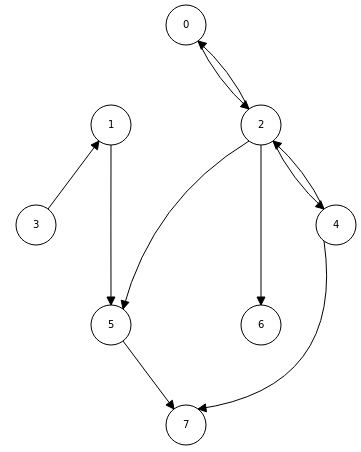
\includegraphics[scale=0.5]{grafin.png}
\end{center}

\begin{enumerate}[label=\Alph*]
	\item (10\%) Complete la representación de \textbf{matrices de adyacencia}. Si no hay arco,
  por simplicidad, deje el espacio en blanco. No coloque ceros.

\begin{center}
\begin{tabular}{| c | c | c | c | c | c | c | c | c |}
\hline
  & 0 & 1 & 2 & 3 & 4 & 5 & 6 & 7 \\
\hline
0 &   &   & 1  &  &   &   &   &   \\
\hline
1 &   &   &   &   &   & 1  &   &   \\
\hline
2 &   &   &   &   &   &   &   &   \\
\hline
3 &   &   &   &   &   &   &   &   \\
\hline
4 &   &   &   &   &   &   &   &   \\
\hline
5 &   &   &   &   &   &   &   &   \\
\hline
6 &   &   &   &   &   &   &   &   \\
\hline
7 &   &   &   &   &   &   &   &   \\ 
\hline
\end{tabular}
\end{center}

	\item (10\%) Complete la representación de \textbf{listas de adyacencia}. Como
  el grafo no tiene pesos, sólo se colocan los sucesores en la lista de adyacencia.
  Los sucesores o vecinos son los vértices a los que se puede llegar a partir de
  un vértice directamente, no transitivamente. \\


$0 \rightarrow [2]$\\
$1 \rightarrow [5]$ \\
$2 \rightarrow$\\
$3 \rightarrow$\\
$4 \rightarrow$\\
$5 \rightarrow$\\
$6 \rightarrow$\\
$7 \rightarrow$\\


\end{enumerate}





\section{Backtracking 30\%}
%http://algorithms.tutorialhorizon.com/backtracking-rat-in-a-maze-puzzle/
Sea un laberinto una matriz de $n \times n$. Una rata tiene que encontrar la ruta para salir. La rata empieza
en la esquina superior izquierda (\texttt{matriz[0][0]}) y debe ir hasta la esquina inferior derecha (\texttt{matriz[N-1][N-1]}) 
para salir del laberinto. Algunas celdas están bloquedas y por esas no puede pasar. La rata se puede mover en cuatro direcciones:
izquierda (\emph{left}), derecha (\emph{right}), abajo (\emph{down}) y arriba (\emph{up}).

La entrada del algoritmo es una matriz donde los valores son cero o uno. Un valor de cero significa que la celda
está bloqueda, y un valor de 1 significa que la celda está libre y la rata se puede mover a esa celda.

La matriz \texttt{solucion} se utiliza para almacenar la solución. Es importante que la rata sepa cuál es el movimiento
inmediatamente anterior para no terminar en un ciclo infinito, por ejemplo, moviéndose izquierda y derecha, sucesivamente,
por siempre. 

\begin{verbatim}
01 boolean findPath(int[][] maze, int x, 
      int y, int N, String direction) {
02    if(x==N-1 && y==N-1){
03      solution[x][y] = 1;
04      return true;
05    }
06    if (......................) {
07      solution[x][y] = 1;     
08      if(direction!="up" && 
       findPath(maze, x+1, y, N, "down")){ 
09        return true; }
10      if(direction!="left" && 
       findPath(maze, x, y+1, N,"right")){ 
11        return true; }
12      if(direction!="down" && 
       findPath(maze, x-1, y, N, "up")){ 
13        return true; }
14      if(direction!="right" &&  
       findPath(....................)){ 
15        return true; }
16      solution[x][y] = 0;
17      return false;
18    }
19    return .............;
20  }
21  public boolean isSafeToGo(int[][] maze, 
                     int x, int y, int N) {
22    if (x >= 0 && y >= 0 && x < N  && 
        y < N && maze[x][y] != 0) {
23      return true;
24    }
25    return false;
26  }
27 }
\end{verbatim}


\begin{enumerate}[label=\Alph*]


    \item (10\%) Completa la línea 6: \\


  \_\_\_\_\_\_\_\_\_\_\_\_\_\_\_\_\_\_\_\_\_\_\_\_


    \item (10\%) Completa la línea 14:\\


  \_\_\_\_\_\_\_\_, \_\_\_\_\_\_\_\_, \_\_\_\_\_\_\_\_, \_\_\_\_\_\_\_\_, \_\_\_\_\_\_\_\_


    \item (10\%) Completa la línea 19:\\


  \_\_\_\_\_\_\_\_\_\_\_\_\_\_\_\_\_\_\_\_\_\_\_\_



\end{enumerate}



  \section{Voraces 10\%}
  Dados dos arreglos de enteros $a$, $b$, de tamaño $n$ cada uno, encuentre dos permutaciones $a'$, $b'$ tal que $\sum\limits_{i = 0}^{n - 1}{|a'_i - b'_i|}$ sea tan pequeño como sea posible.

{\footnotesize
  \textbf{Nota: } En Java, \texttt{Math.abs(n)} calcula el valor absoluto de $n$.
  \begin{lstlisting}
  int solve(int[] a, int[] b){
    int n = a.length;
    //Paso 1: Procesamiento inicial
    ..............;
    ..............;
    int res = -1;
    for(int i = 0; i < n; ++i){
      //Desicion voraz
      res += Math.abs(a[i] - b[i]);
    }
    return res;
  }
  \end{lstlisting}
  }

  \begin{enumerate}[label=\alph*]
    % Respuesta: Arrays.sort(a), Arrays.sort(b)
    \item (10\%) Complete las líneas 4, 5\\

     ..............., ............

  \end{enumerate}








\end{document}